\documentclass[tikz,border=4pt]{standalone}
\usepackage{amsmath,amssymb}
\usepackage{pgfplots}\pgfplotsset{compat=1.18}\usepgfplotslibrary{polar}
\usetikzlibrary{arrows.meta,positioning,automata,shapes,shapes.misc,calc,decorations.pathmorphing,decorations.markings,angles,quotes,patterns,mindmap,matrix,knots,hobby,trees}
\tikzset{->-/.style={decoration={markings, mark=at position 0.5 with {\arrow{Stealth}}}, postaction={decorate}}}
\begin{document}
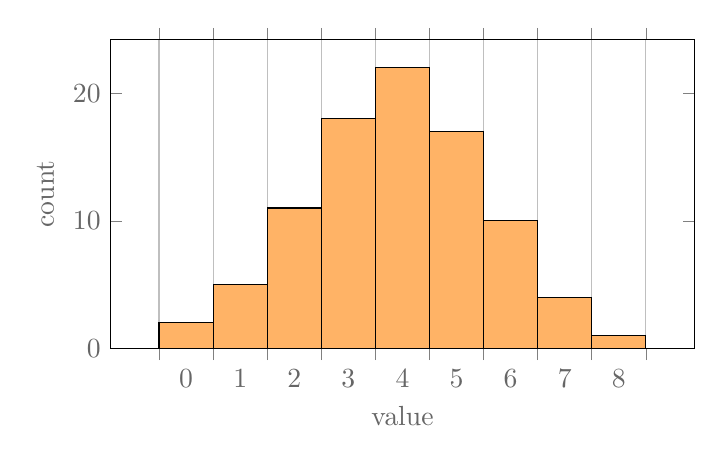
\begin{tikzpicture}
\begin{axis}[ybar interval, ymin=0, width=9cm, height=5.5cm, xlabel={value}, ylabel={count}, fill opacity=0.6]
\addplot[fill=orange] coordinates {(0,2) (1,5) (2,11) (3,18) (4,22) (5,17) (6,10) (7,4) (8,1) (9,0)};
\end{axis}
\end{tikzpicture}
\end{document}
